\subsection{Целевые функционалы и выходные величины}

Решение уравнения Рейнольдса даёт поле давления $p(s_1, s_2, t)$
в смазочном слое. По найденному давлению и известной геометрии
зазора $h(s_1, s_2, t)$ вычисляются интегральные характеристики узла,
определяющие его работоспособность и энергоэффективность.
В настоящем подразделе приведены унифицированные формулы
для всех трёх постановок (2.1.2-2.1.4).

Элемент площади $dA$ для каждой постановки:
\begin{itemize}
  \item упорная (2.1.2): $dA = r\,dr\,d\theta$,\quad
        $r \in [R_{\mathrm{in}},\,R_{\mathrm{out}}]$,\;
        $\theta \in [0,\,2\pi]$;
  \item радиальная (2.1.3): $dA = R\,d\theta\,dz$,\quad
        $\theta \in [0,\,2\pi]$,\; $z \in [0,\,L]$;
  \item возвратно-поступательная (2.1.4): $dA\!=\!R\,d\theta\,dz$,\,
        $\theta\!\in\![0,\,2\pi]$,\, $z\!\in\![0,\,L]$.
\end{itemize}

%% ===== Блок 1: Несущая способность =====
\subsubsection*{Несущая способность}

Для упорного подшипника результирующая нагрузка направлена вдоль оси
вращения и является скалярной величиной:
\begin{equation}
  W = \iint_A p\,dA
    = \int_0^{2\pi}\!\int_{R_{\mathrm{in}}}^{R_{\mathrm{out}}}
      p(r,\theta)\,r\,dr\,d\theta.
  \label{eq:func_W_thrust}
\end{equation}

Для радиального и возвратно-поступательного подшипников давление
распределено по цилиндрической поверхности, поэтому результирующая
сила имеет две компоненты в плоскости поперечного сечения.
Нормаль к поверхности вала направлена радиально наружу:
$\mathbf{n} = (\cos\theta,\,\sin\theta)$.
Гидродинамическая сила, действующая на вал со стороны смазочного слоя,
определяется как:
Поскольку давление действует на поверхность вала по направлению
внутрь ($d\mathbf{F} = -p\,\mathbf{n}\,dA$), компоненты силы
содержат знак <<минус>>:
\begin{equation}
\begin{alignedat}{2}
  & F_x(t) &\;=\;& -\int_0^L \int_0^{2\pi}
    p(\theta,z,t)\,\cos\theta\;R\,d\theta\,dz, \\
  & F_y(t) &\;=\;& -\int_0^L \int_0^{2\pi}
    p(\theta,z,t)\,\sin\theta\;R\,d\theta\,dz, \\
  & F(t)   &\;=\;& \sqrt{F_x^2(t) + F_y^2(t)}.
\end{alignedat}
  \label{eq:func_F_components}
\end{equation}
Здесь ось $x$ соответствует направлению $\theta = 0$,
ось $y$ -- направлению $\theta = \pi/2$.
Угол нагружения (attitude angle):
\begin{equation}
  \psi(t) = \mathrm{atan2}\bigl(F_y(t),\,F_x(t)\bigr).
  \label{eq:func_psi}
\end{equation}

Угол $\psi$ определяет направление результирующей гидродинамической
силы относительно оси $x$ и используется при анализе орбит вала
(главы~5-8).
Для стационарного радиального подшипника зависимость от $t$ отсутствует.
Схема компонент силы показана на рис.~\ref{fig:force_components}.

% [РИСУНОК: Компоненты гидродинамической силы]
\begin{figure}[!ht]
\centering
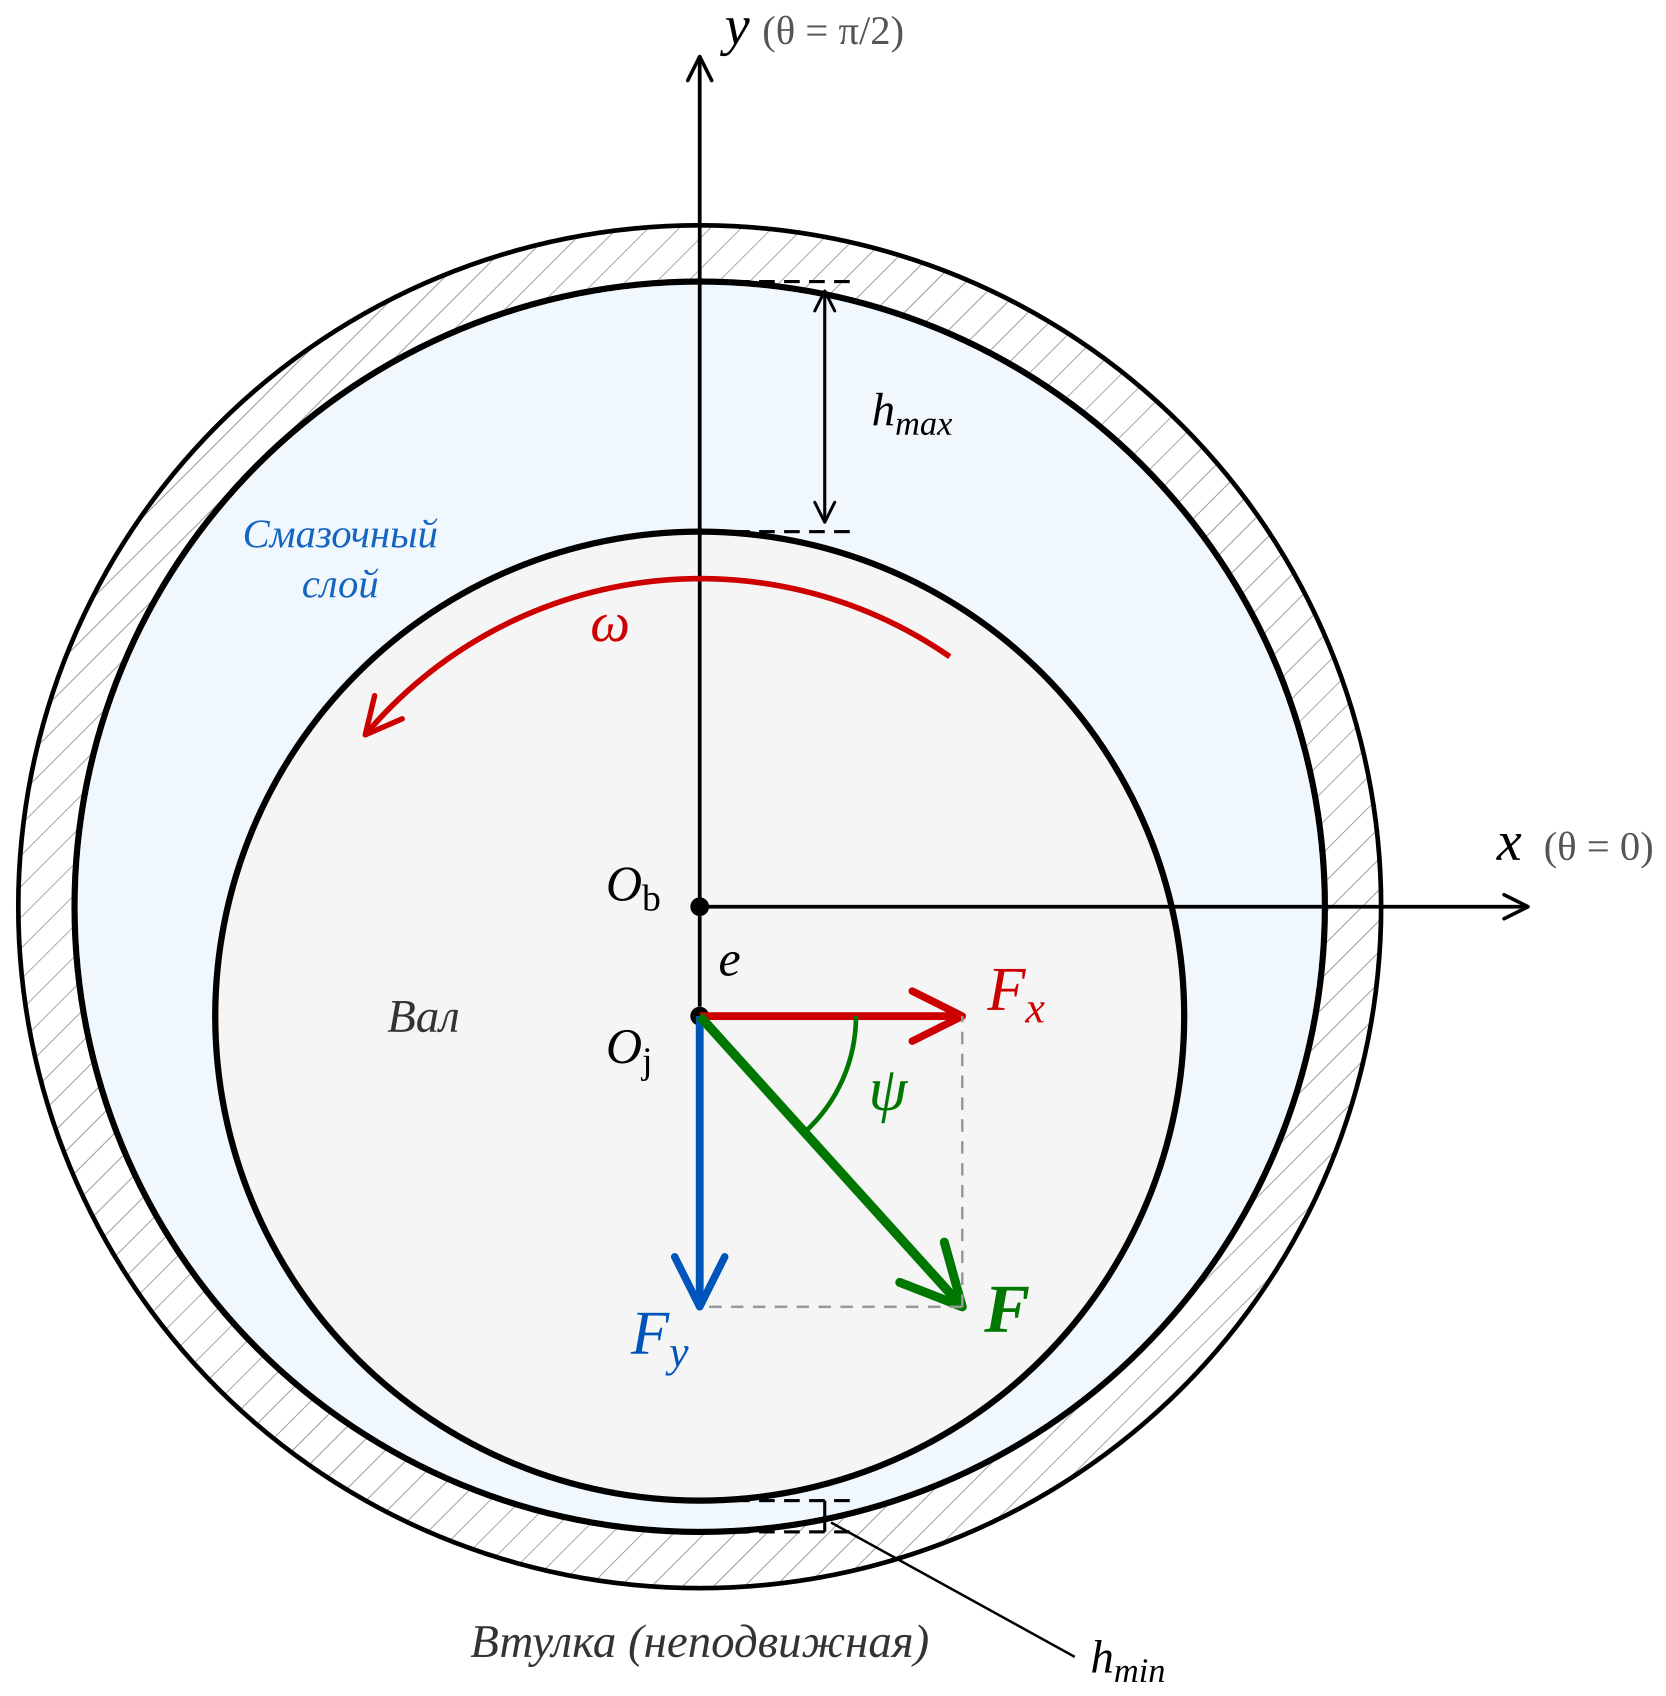
\includegraphics[width=\textwidth,height=0.9\textheight,keepaspectratio]{figures/ch02/fig_2_10.png}
\caption{Компоненты гидродинамической силы на валу/плунжере}
\label{fig:force_components}
\end{figure}

%% ===== Блок 2: Расходы и утечки =====
\subsubsection*{Расходы и утечки}

Удельные потоки $q$ определены в соответствующих постановках
(см.~\eqref{eq:thrust_q_r}, \eqref{eq:journal_q_z},
\eqref{eq:recip_q_z}).
Здесь приводятся только интегральные расходы через границы
рабочей зоны.

Упорный подшипник -- суммарные объёмные расходы через наружную
и внутреннюю кромки (см.~также~\eqref{eq:thrust_Q_radial}):
\begin{equation}
\label{eq:func_Q_thrust}
\begin{split}
  &Q_{\mathrm{out}} = \int_0^{2\pi}
    q_r(R_{\mathrm{out}},\theta)\,R_{\mathrm{out}}\,d\theta, \\
  &Q_{\mathrm{in}} = \int_0^{2\pi}
    q_r(R_{\mathrm{in}},\theta)\,R_{\mathrm{in}}\,d\theta.
\end{split}
\end{equation}

Радиальный подшипник -- утечки через торцы
(см.~также~\eqref{eq:journal_Q_side}):
\begin{equation}
  Q_{\mathrm{out}} = \int_0^{2\pi}
    q_z(\theta,L)\,R\,d\theta,
  \quad
  Q_{\mathrm{in}} = \int_0^{2\pi}
    q_z(\theta,0)\,R\,d\theta.
  \label{eq:func_Q_journal}
\end{equation}

Возвратно-поступательный подшипник -- мгновенные расходы через
обе границы и их усреднение по периоду
(см.~также~\eqref{eq:recip_Q_leakage}):
\begin{equation}
  Q_{\mathrm{out}}(t) = \int_0^{2\pi}
    q_z(\theta,L,t)\,R\,d\theta,
  \quad
  Q_{\mathrm{in}}(t) = \int_0^{2\pi}
    q_z(\theta,0,t)\,R\,d\theta,
  \label{eq:func_Q_recip}
\end{equation}
\begin{equation}
  \langle Q_{\mathrm{out}} \rangle
    = \frac{1}{T}\int_0^T Q_{\mathrm{out}}(t)\,dt,
  \quad
  \langle Q_{\mathrm{in}} \rangle
    = \frac{1}{T}\int_0^T Q_{\mathrm{in}}(t)\,dt,
  \label{eq:func_Q_recip_avg}
\end{equation}
где $T = 2\pi/\Omega$ -- период возвратно-поступательного движения.

Положительный $Q_{\mathrm{out}}$ соответствует вытеканию смазки
из рабочей зоны, что согласуется с конвенцией, принятой
в подразделах~2.1.2-2.1.4.

%% ===== Блок 3: Трение, момент трения, потери мощности =====
\subsubsection*{Сила и момент трения}

Касательное напряжение вдоль направления увлечения $s_1$
следует из профиля скорости~\eqref{eq:velocity_profile_u}.
Первое слагаемое -- вязкое (куэттовское), второе -- давленческое
(пуазейлевское).
Выражения для касательного напряжения на подвижной ($y = h$)
и неподвижной ($y = 0$) поверхностях:
\begin{equation}
  \tau\big|_{y=h} = \frac{\mu\,U}{h}
    + \frac{h}{2}\,\frac{\partial p}{\partial s_1},
  \quad
  \tau\big|_{y=0} = \frac{\mu\,U}{h}
    - \frac{h}{2}\,\frac{\partial p}{\partial s_1}.
  \label{eq:func_tau_both}
\end{equation}

Далее при вычислении момента и силы трения используется напряжение
на неподвижной поверхности $\tau|_{y=0}$, что даёт силу сопротивления
движению.

Конкретизация производной $\partial p/\partial s_1$ и скорости $U$
для каждой постановки:
\begin{itemize}
  \item радиальная: $s_1 = R\theta$ $\Rightarrow$
        $\partial p/\partial s_1 = (1/R)\,\partial p/\partial\theta$,\;
        $U = \omega R$;
  \item упорная: $s_1 = r\theta$ $\Rightarrow$
        $\partial p/\partial s_1 = (1/r)\,\partial p/\partial\theta$,\;
        $U = \omega r$;
  \item возвратно-поступательная: $s_1 = z$ $\Rightarrow$
        $\partial p/\partial s_1 = \partial p/\partial z$,\;
        $U = U(t)$.
\end{itemize}

В приведённых ниже интегралах $\tau$ обозначает касательное
напряжение на неподвижной поверхности $\tau|_{y=0}$.

Момент трения для упорного подшипника:
\begin{equation}
  M_f = \int_0^{2\pi}\!\int_{R_{\mathrm{in}}}^{R_{\mathrm{out}}}
    \tau(r,\theta)\,r^2\,dr\,d\theta.
  \label{eq:func_Mf_thrust}
\end{equation}

Момент трения для радиального подшипника:
\begin{equation}
  M_f = \int_0^L\!\int_0^{2\pi}
    \tau(\theta,z)\,R^2\,d\theta\,dz.
  \label{eq:func_Mf_journal}
\end{equation}

Сила трения для возвратно-поступательного подшипника:
\begin{equation}
  F_f(t) = \int_0^L\!\int_0^{2\pi}
    \tau(\theta,z,t)\,R\,d\theta\,dz.
  \label{eq:func_Ff_recip}
\end{equation}

Потери мощности на трение для вращательных постановок:
\begin{equation}
  P_f = M_f \cdot \omega.
  \label{eq:func_Pf_rot}
\end{equation}

При принятой конвенции (касательное напряжение на неподвижной
поверхности) величины $M_f$ и $F_f$ представляют сопротивление
движению, и потери мощности $P_f \geq 0$.

Для возвратно-поступательной постановки мощность потерь является
функцией времени:
\begin{equation}
  P_f(t) = |F_f(t) \cdot U(t)|,
  \quad
  \langle P_f \rangle = \frac{1}{T}\int_0^T P_f(t)\,dt.
  \label{eq:func_Pf_recip}
\end{equation}

Модуль обеспечивает неотрицательность потерь при смене направления
скорости.

%% ===== Блок 4: Минимальная толщина плёнки =====
\subsubsection*{Минимальная толщина плёнки}

\begin{equation}
  h_{\min}(t) = \min_{(s_1,\,s_2)\,\in\,\Omega}\,h(s_1,s_2,t).
  \label{eq:func_hmin}
\end{equation}

Минимальная толщина плёнки -- критический параметр работоспособности:
при $h_{\min} \to 0$ нарушается режим жидкостного трения.
Для стационарных задач $h_{\min}$ является числом,
для нестационарных -- функцией времени.
Дополнительно может представлять интерес максимальное давление
$p_{\max}(t) = \max_\Omega p$.

%% ===== Блок 5: Коэффициент трения =====
\subsubsection*{Коэффициент трения}

Безразмерный коэффициент трения для радиального
и возвратно-поступательного узлов:
\begin{equation}
  f(t) = \frac{|F_f(t)|}{F(t)}.
  \label{eq:func_f}
\end{equation}

Для упорного подшипника естественнее определять коэффициент трения
через момент:
\begin{equation}
  f_T = \frac{M_f}{W \cdot R_m},
  \quad
  R_m = \frac{R_{\mathrm{in}} + R_{\mathrm{out}}}{2}.
  \label{eq:func_fT}
\end{equation}

%% ===== Завершающий абзац =====

Введённые функционалы определяют основные цели при анализе
и оптимизации подшипников скольжения:
\begin{itemize}
  \item максимизация несущей способности $W$ (или $F$);
  \item минимизация потерь на трение $P_f$ (или $M_f$);
  \item минимизация утечек $Q_{\mathrm{out}}$;
  \item обеспечение $h_{\min}$ выше критического порога
        (предотвращение сухого контакта)~\cite{sfyris2012,chasalevris2012,chasalevris2013}.
\end{itemize}
Для нестационарных задач (подраздел~2.1.4) анализ проводится
как для мгновенных значений, так и для усреднённых по периоду
$\langle \cdot \rangle$.
